\cleardoublepage
\chapter{Statistical Distributions}\label{chap:app4}

Much of the problems in physics can be described, at least approximately, with a small group of theoretical statistical distributions characterized by a \textbf{\textit{probability density function $P(x)$}}, which provides the expected frequency of a particular random event happening.

This appendix will proceed to explain the salient features of the statistical distributions to which the data taken in this experiment fit. In particular, the \textbf{Normal or Gaussian} distribution, the \textbf{Poisson} distribution and the \textbf{Chi-square} distribution are discussed.


\section{Normal or Gaussian distribution}\label{sec:gauss}

Most natural phenomena fit a Gauss \enquote{bell} curve, so is also known as \textit{Normal Distribution}. Accurately describe any population whose randomness is due to an effect that can be decomposed into the sum of a large number of independent causes. It applies to a population of CONTINUOUS random variable. Instrumental errors are well described by a Gaussian curve.

The Gaussian distribution is a mathematical simplification of the  \textbf{\textit{Bernoulli or Binomial Distribution}} when the number of trials $N$ is very large ($\gg$ 30). The probability that in each test the obtained value is one of two given values is not very small potential ($\geq$ 0.05). The probability of obtaining a value $x$ is:

	\be P(x) = \frac{1}{\sigma\sqrt{2\pi}} \,e^{\frac{\left(x-\mu \right)^2}{2\sigma^2}}\ee

where $\mu$ is the mean and $\sigma$ the standard deviation, which is the width of the distribution at $\sim$60\% of the overall height, although sometimes the full width at half height is used: FWHM = 2.35$\sigma$. This distribution is CONTINUOUS, SYMMETRICAL around the mean value, and NORMALIZED with TWO parameters, $\mu$ and $\sigma^2$.

We must clarify that the expected value of the random variable $x$ is defined as: $E [x] = \int x \,P(x) \,dx = \,<x>$ and is also called \textit{average} or \textit{mean value} of $x$, which is usually denoted as: $\mu = E [x]$, and refers to the theoretical distribution $P(x)$, so it should not be confused with the average experimental value of a sample that is mentioned in Appendix \ref{chap:app3}.

This distribution is centered in $\mu$, where it has its maximum. It normalization factor is $1/\sigma\sqrt{2\pi}$ so that the integral of $P(x)$ in the entire sample space is 1, and its width is given by $1/2\sigma^2$, so that the bigger the $\sigma$, the greater the width. The two inflection points are given by $\mu \pm \sigma$. The usual notation is $N(\mu, \sigma)$.

Important parameters:
	\bi
		\item $\left\langle x \right\rangle = \mu$ mean (matches mode).
		\item $\left\langle(x - \mu)^2\right\rangle = \sigma^2 = \bar{x^2} - \mu^2$ variance.
		\item $\sigma$ Standard deviation.
	\ei

The probability of obtaining a value of $x$ less than one particular $x_c$ is given by the integral:

	\be P(x < x_c) = \int_{-\infty}^{x_c} P(x) \,dx \ee

As this integral is difficult to solve, the following approximation is used:

	\be P(x < x_c) = 1 - \frac{1}{\sqrt{2}\pi} \,e^{-\frac{1}{2}\left( \frac{x_c - \mu}{\sigma}\right)^2} \left[ a_1t + a_2t^2 + a_3t^3 + a_4t^4 + a_5t^5\right] \ee\vfill

\bc
\begin{minipage}[t]{.4\textwidth}
	\bc with\ec
	\begin{equation*}
		t = \frac{1}{1 + a_0 \left(\frac{x_c - \mu}{\sigma}\right)}
	\end{equation*}
\end{minipage}%
\begin{minipage}[t]{.6\textwidth}
	\bc and\ec
	\begin{equation*}
		\begin{split}
			a_0 &= \text{0.2316419}   \\
			a_1 &= \text{0.31938153}  \\
			a_2 &= -\text{0.356563782}\\
		\end{split}\quad
		\begin{split}
			a_3 &= \text{1.78147937}  \\
			a_4 &= -\text{1.821255978}\\
			a_5 &= \text{1.330274429} \\
		\end{split}
	\end{equation*}
\end{minipage}
\ec

A similar approach is used in the program used to calculate the confidence level of $\chi^2$. See the code at the end of this appendix.

	\bfi[H]
		\bc
			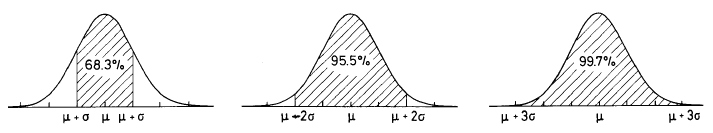
\includegraphics[width=.9\textwidth]{img/app41.png}
			\caption
				[Confidence intervals.]
				{Confidence intervals:\\
					$x = \mu \pm  \sigma \rightarrow$ 68.3\% ($\sim$2/3 of the data)\\
					$x = \mu \pm 2\sigma \rightarrow$ 95.4\%\\
					$x = \mu \pm 3\sigma \rightarrow$ 99.7\%.}\label{fig:confidence}
		\ec
	\efi


	

\section{Poisson distribution}\label{sec:poisson}

Sometimes an observation consists of counting objects. We always count in relation to a range that can be time, length, area, etc.

The Poisson distribution applies to \enquote{rare} events. It describes DISCRETE  processes in which the observation of a single event is very unlikely, but the number of trials is so large that at the end there is a reasonable number of events.

It is also considered to be a limit of the Binomial distribution when the number of trials is very large and the probability of each test the obtained value is one of two possible values is very small. For example, in radioactive decay, if small time-measurement intervals are taken and compared with the average life of the source, where the number of nuclei $N$ is large, the probability of getting a value $x$ times can be obtained as follows:

\bi
	\item Probability of having an event per unit interval: $\lambda$ (very small).
	\item Probability of having an event within an interval $dt$: $\lambda \,dt$.
	\item In an interval $t$, the average of events is: $\mu = \lambda t$.
\ei

The basic assumption is that the $\lambda$ probability is so small that in the interval $dt$ two or more events can not occur:

\bi
	\item Chance of having 2 events within a time interval $dt$: $p_2 (dt) = O$.
	\item Probability to have O events within a time interval $dt$: $p_0 (dt) = 1 - \lambda \,dt$.
	\item Probability of having $x$ events within an interval $t + dt$:\\
 $p_x (t + dt) = p_x (t) (1 - \lambda \,dt) + p_{x-1} (t) \,\lambda \,dt$.
\ei


If now we subtract $p_x (t)$ on both sides of the last expression we obtain:

\be
	\begin{split}
		\frac{dp_x(t)}{dt} = &\lambda\left( p_{x-1} - p_x \right)	\quad
		\rightarrow	p_x = \frac{\left(\lambda t \right)^x}{x!} \,e^{\lambda t}\\
		&P(x) = \frac{\mu^x}{x!}e^\mu					\quad
		x = 0, 1, 2 \dots
	\end{split}
\ee

This would be the probability that the random variable takes the value $x$. This distribution is DISCRETE, NORMALIZED and ASYMMETRIC with respect to the mean, with a SINGLE parameter, $\mu$.

Important parameters:
	\bi
		\item $\mu = \overset\infty{\underset 0{\sum}} x P(x)$ mean (matches mode).
		\item $\sigma^2 = x^2 - \mu^2$ variance.
		\item $\sigma = \sqrt{\mu}$ Standard deviation.
	\ei


This indicates that if random events are counted, it is very difficult to obtain high accuracy. For a $\sigma\sim$1\%, 10,000 events would be needed. When we perform an experiment of counting random events and obtain a value $x$, the result with its error is: $x ± \sqrt{x}$.

If the average is increased, the probability distribution moves to the right and its shape becomes more symmetric and flat. When the numbers are large, the Poisson distribution becomes a Gaussian distribution with $\sigma = \sqrt{\mu}$, so we have a particular case of Gaussian that depends on a single parameter: the mean $\mu$.

	\bfi[H]
		\bc
			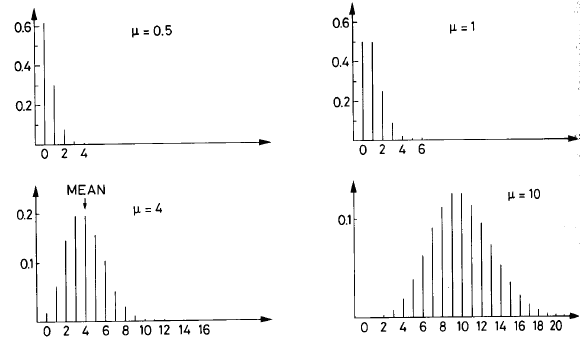
\includegraphics[width=.9\textwidth]{img/app42.png}\\
			\caption
				[Limit of a Gaussian distribution.]
				{The limit of a Poisson distribution is a Gaussian:\\
				${\color{white}.} \qquad {\color{white}.} \qquad P(x) = \frac{1}{\sqrt{2\pi\mu}} \,e^{\frac{(x - \mu)^2}{2\mu}} $\\
This result is very important because it indicates that the result of having a large number of events is no different from the result of measuring a continuous variable.}\label{fig:poisson}
		\ec
	\efi

The probability of obtaining a value of $x$ that is lower than one particular $x_c$ is given by the sum:

	\be P(x \leq x_c) = \sum_0^{x_c} \frac{\mu^k}{k!} \,e^\mu \ee

The values ​​of the Poisson distribution function calculated with this expression are shown in the following tables:

	\bfi[H]
		\bc
			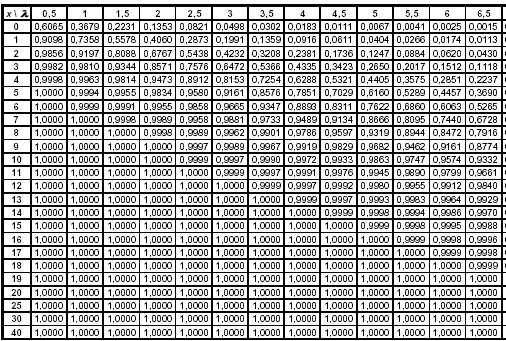
\includegraphics[width=.9\textwidth]{img/app43.png}\\[12pt]
			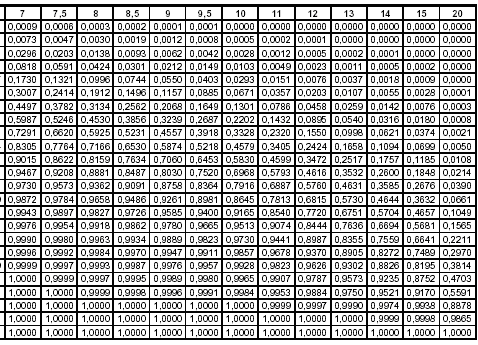
\includegraphics[width=.9\textwidth]{img/app44.png}\\
			\caption
				[Limit of a Gaussian distribution.]
				{Values ​​of the Poisson distribution for a certain value of $x$ and for a given value of the mean (here designated by $\lambda$).}\label{tab:tables}
		\ec
	\efi

\section{Chi-squared distribution}\label{sec:chi2}

It is particularly useful for estimating the so called \textit{goodness} of the fit of the experimental data when compared with the theoretical distribution formulas.

The shape of this distribution is deducted below: Suppose there are $n$ independent variables $x_i$ with \textit{normal} distributions of mean values $\mu_i$ and ​​standard deviations $\sigma_i$,  with:

	\be \chi^2 = \sum_i^n \frac{(x_i - \mu_i)^2}{\sigma^2}\ee

The probability that $x_i$ is between $x_i$ and $dx_i$ is:

	\be
		\begin{split}
			P(x_1x_2\dots x_n) \,dx_1 \,dx_2\dots\,dx_n 
			&= P(x_1)P(x_2)\dots P(x_n) \,dx_1 \,dx_2\dots\,dx_n \\
			&= \frac{1}{\sigma_1\sigma_2\dots\sigma_n(2\pi)^{n/2}} \,e^{-\frac{\chi^2}{2}}
		\end{split}
	\ee

The probability that $\chi^2$ 
is between $\chi^2$ and $\chi^2 + \,d\chi^2$ 
is $e^{-\frac{\chi^2}{2}}\chi^{n-1} \,d\chi$, 
where $\chi^{n-1} \,d\chi$ 
is the volume between two spheres of radius $\chi^2 + \,d\chi^2$ 
in an n-dimensional space. Manipulating this expression, integrating over all space to find the normalization constant, and replacing $n$ by $\nu$ (the degrees of freedom) we obtain:

	\be
		P(\chi^2) = \frac{\left(\frac{\chi^2}{2}\right)^{\frac{\nu}{2}-1}}%
						 {2\Gamma\left(\frac{\nu}{2}\right)}% 
					e^{-\frac{\chi^2}{2}}
	\ee

where $\Gamma$ is the Gamma function of Euler, which is defined as:

	\be
		\Gamma\left(\frac{\nu}{2}\right) =
		\left\{%
			\begin{array}{l}
				\left(\frac{\nu}{2}-1\right)!\\
				\sqrt{\pi}
				\left(\frac{1}{2}\right)
				\left(\frac{3}{2}\right) \dots 
				\left(\frac{\nu}{2} - 1\right)
			\end{array}
			\quad
			\begin{split}
				&\text{ for\ even\ }\nu\\
				&\text{ for\ odd\  }\nu
			\end{split}
		\right.
	\ee

	\bfi[H]
		\bc
			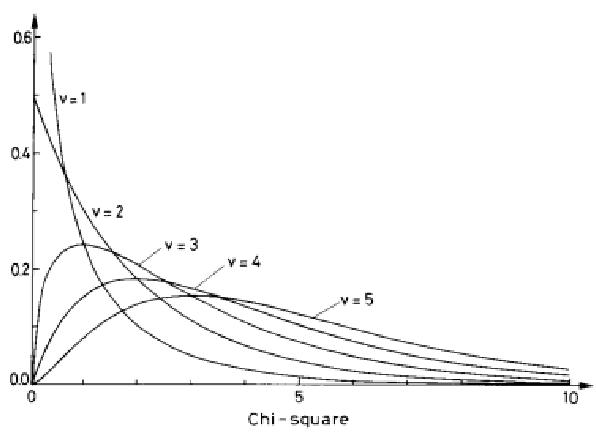
\includegraphics[width=.9\textwidth]{img/app45.png}
			\caption
				[Chi-squared distribution.]
				{Chi-squared distribution.}\label{fig:chi2}
		\ec
	\efi

This distribution is ASSYMETRIC, with a SINGLE paremeter $\nu$ that determines the shape of the distribution.

Important parameters:
	\bi
		\item $\chi^2 = n - 2$ most probable value.
		\item $\mu = \,<\chi^2> = n$ mean value.
		\item $\sigma^2 = 2n$ variance.
		\item $\sigma(\chi^2) = \sqrt{2n}$ standard deviation.
	\ei

If the variables are not independent, $n$ is changed by $\nu = n - k$, where $\nu$ represents the degrees of freedom, and $k$ is the number of constraints in the system.

The $\chi^2$ of a fit has a $\chi^2$ distribution with $\nu$ degrees of freedom and a constraint, which can be rewritten as:

	\be\chi^2 = \frac{(n-1)s^2}{\sigma^2}\ee

where $s^2$ is the best sample estimate of the population variance of the $n$ variables, and:

	\be \sigma(s^2) = \sqrt{\frac{2}{n - 1}} \sigma^2 \ee

is the standard deviation of the sample variance $s^2$ if $\sigma^2$ is known for a normal universe.

The probability of obtaining a value of $\chi^2$ that is lower than one particular $\chi_c^2$ is given by the integral:

	\be
		P\left(\chi^2 < \chi_c^2\right) =
		\int_{-\infty}^{\chi_c^2} P_\nu(x) \,dx
	\ee

Since this integral is very difficult to solve, this approximation used instead:

	\be
		\begin{split}
			P\left(\chi^2 < \chi_c^2\right) &= \frac{2\chi_c^2}{\nu} P_\nu(\chi^2)
			\left[1 + \sum_{k=1}^\infty \frac{\chi^{2k}}{(\nu + 2)(\nu + 4)\dots(\nu + 2k)}\right]\\[12pt]
			Q\left(\chi^2 < \chi_c^2\right) &= 1 - P(\chi^2 < \chi_c^2)
		\end{split}
	\ee

If we pick a particular $\chi_c^2$ and compare it with the $\chi^2$ of the fit to be evaluated, three cases can occur:

\bi
	\item If $\chi^2 \in [0, \chi_c^2)$ it is possible to say that the fit is good,
	\item If $\chi^2 \in [\chi_c^2, \infty)$ it is bad,
	\item If $\chi^2 = \chi_c^2$ this criteria doesn not decide.
\ei


In addition, the judgment made deserve a certain confidence as a percentage that must be previously chosen. If we choose a confidence level of 95\%, 0.05 is the probability of being wrong, \textit{i.e.}: one time in 20.

	\ctable [
	cap	    = {Probability that the $\chi_c^2$ of the fit is between the values ​​indicated by P and Q.},
 	caption = {For different values ​​of $\chi_c^2$, the table shows the values ​​of the probability that the $\chi_c^2$ of the fit is between the values ​​indicated by P and Q. This table is presented for guidance only, as a bad result may be obtained by chance even if the fit was good.},
 	label   = {tab:chi},
 	pos	    = H,
	botcap
	]
	{c c c}
	{}
 	{\FL
		\textbf{$\chi_c^2$} &
		\textbf{P$\left(\chi^2 < \chi_c^2\right)$} &
		\textbf{Q$\left(\chi^2 < \chi_c^2\right)$}\\
		$\nu + $3$\sqrt{\text{2}\nu}$ & 0.99     & 0.01 \\
		$\nu + $2$\sqrt{\text{2}\nu}$ & 0.96     & 0.04 \\
		$\nu + \sqrt{\text{2}\nu}$    & 0.85     & 0.15 \\
		$\nu$                         & 0.5--0.6 & 0.5--0.4
	\LL}


\bi
	\item If the Normal distribution is applied:
The probability density of finding $x_1, \dots, x_n$ as values ​​of the random variable $x$ of a population with normal distribution $N(\mu, \sigma)$ is:

	\bc $P(x_1, \dots, x_n) = \frac{1}{\sigma^n(2\pi)^{n/2}}e^{-\frac{\chi^2}{2}} \qquad $
	with
		$\qquad \chi^2 = \overset n{\underset i{\sum}} \frac{(x_i - \bar{x})^2}{\sigma_i^2}$
	\ec

	\graybox{.9}{.75}{
		\bc\textcolor{gray}{\Large{\sffamily Special case: Weighted averages}}\ec

		Suppose we have $x_1 \in N(\bar{x}, \sigma_1)$  and $x_2 \in N(\bar{x}, \sigma_2)$. The probability density of obtaining $x_1$ and $x_2$ is:

	\bc $P(x_1, x_2) = \frac{1}{2\pi\sigma_1\sigma_2}e^{-\frac{\chi^2}{2}}$\\[12pt]
	where,\\[12pt]
	$\chi^2 =  \frac{(x_1 - \bar{x})^2}{\sigma_1^2} + \frac{(x_2 - \bar{x})^2}{\sigma_2^2}$
	\ec

	\bc $\frac{d\chi^2}{d\bar{x}} \qquad \rightarrow \qquad 
		\bar{x} = \frac { \frac{x_1}{\sigma_1^2} + \frac{x_2}{\sigma_2^2} }
						{ \frac{1}{\sigma_1^2}   + \frac{1}{\sigma_2^2}}$
	\ec
	}
	\graybox{.9}{.75}{


When there are several data, the procedure is similar, and in general we obtain:

	\begin{minipage}{.5\textwidth}
		WEIGHTED AVERAGE
	\end{minipage}\begin{minipage}{.5\textwidth}
		$\bar{x} = \frac{ \underset i{\sum}w_ix_i }{ \underset i{\sum}w_i }$
	\end{minipage}
	\begin{minipage}{.5\textwidth}
		ERROR\\(STANDARD DEVIATION)
	\end{minipage}\begin{minipage}{.5\textwidth}
		$S = \frac{ 1 }{ \sqrt{\underset i{\sum}w_i} }$
	\end{minipage}

	\begin{minipage}{.5\textwidth}
		WEIGHTS
	\end{minipage}\begin{minipage}{.5\textwidth}
		$w_i = \frac{1}{\sigma_i^2}$
	\end{minipage}

	}

	\item For the Poisson distribution, we have $\sigma_i^2 = e_i$, $(o_i - e_i)^2 = \sigma_i^2 = e_i$, $\left\langle \chi^2 \right\rangle =$ number of degrees of freedom $= n - 1$. If the result of $\chi^2$ is around the number of degrees of freedom, we have a good agreement; although it could be good and by chance $\chi^2$ be much larger or smaller than this value.
\ei

To evaluate $\chi^2$ use Table \ref{tab:chieval}.


To calculate the level of confidence of the $\chi^2$ of a fit using the $\chi^2$ and the number of constraints, the program \code{cl.cpp} (in C++ language) can be used. The code is shown below.\\[12pt]

\lstinputlisting{../cl/cl.cpp}

A summary of the main differences between the Gaussian, Poisson and Chi-Squared distributions is shown in Table \ref{tab:diffs}.

	\ctable [
	cap	    = {Differences between distributions.},
 	caption = {Differences between distributions.},
 	label   = {tab:diffs},
 	pos	    = H,
	botcap
	]
	{c c c }
	{}
 	{\FL
		\textbf{GAUSS} &
		\textbf{POISSON} &
		\textbf{CHI-SQUARED}\\
		Continuous Variable &
		Discrete Variable &
		Continuous Variable \\
		Symmetric &
		Non-symmetric &
		Non-symmetric \\
		Two parameters ($\mu$, $\sigma$) &
		One parameter ($\mu$) &
		One parameter ($\nu$)
	\LL}



\begin{landscape}

	\ctable [
	cap	     = {Comparison table for $\chi^2$.},
	caption  = {Values ​with which $\chi^2$ ​must be compared for the different degrees of freedom $\nu$ shown in the first column, and for the different levels of confidence shown in the first row.},
	label    = {tab:chieval},
 	pos	     = H,
	doinside = \scriptsize 
	]
	{c c c c c
	 c c c c c
	 c c c c c}
	{}
 	{\FL
		$\nu$ &
		\textbf{.99} & \textbf{.98} & \textbf{.95} & \textbf{.90} &
		\textbf{.80} & \textbf{.70} & \textbf{.50} & \textbf{.30} &
		\textbf{.20} & \textbf{.10} & \textbf{.05} & \textbf{.02} &
		\textbf{.01} & \textbf{.001} \\
 		\textbf{1} & .00016 & .00063 & .0039 & .016  & .064  & .15   & .46  & 1.07   & 1.64   & 2.71  & 3.84  & 5.41  & 6.64  & 10.83 \\ 
		\textbf{2}  & .02  & .04  & .10   & .21   & .45   & .71   & 1.39 & 2.41   & 3.22   & 4.60  & 5.99  & 7.82  & 9.21  & 13.82 \\ 
		\textbf{3}  & .12  & .18  & .35   & .58   & 1.00  & 1.42  & 2.37 & 3.66   & 4.64   & 6.25  & 7.82  & 9.84  & 11.34 & 16.27 \\
		\textbf{4}  & .30  & .43  & .71   & 1.06  & 1.65  & 2.20  & 3.36 & 4.88   & 5.99   & 7.78  & 9.49  & 11.67 & 13.28 & 18.46 \\
		\textbf{5}  & .55  & .75  & 1.14  & 1.61  & 2.34  & 3.00  & 4.35 & 6.06   & 7.29   & 9.24  & 11.07 & 13.39 & 15.09 & 20.52 \\
		\textbf{6}  & .87  & 1.13 & 1.64  & 2.20  & 3.07  & 3.83  & 5.35 & 7.23   & 8.56   & 10.64 & 12.59 & 15.03 & 16.81 & 22.46 \\
		\textbf{7}  & 1.24 & 1.56 & 2.17 & 2.83 & 3.82 & 4.67 & 6.35 & 8.38 & 9.80 & 12.02 & 14.07 & 16.62 & 18.48 & 24.32 \\
		\textbf{8}  & 1.65 & 2.03 & 2.73 & 3.49 & 4.59 & 5.53 & 7.34 & 9.52 & 11.03 & 13.36 & 15.51 & 18.17 & 20.09 & 26.12 \\
		\textbf{9}  & 2.09 & 2.53 & 3.32 & 4.17 & 5.38 & 6.39 & 8.34 & 10.66 & 12.24 & 14.68 & 16.92 & 19.68 & 21.67 & 27.88 \\
		\textbf{10} & 2.56 & 3.06 & 3.94 & 4.86 & 6.18 & 7.27 & 9.34 & 11.78 & 13.44 & 15.99 & 18.31 & 21.16 & 23.21 & 29.59 \\
		\textbf{11} & 3.05 & 3.61 & 4.58 & 5.58 & 6.99 & 8.15 & 10.34 & 12.90 & 14.63 & 17.28 & 19.68 & 22.62 & 24.72 & 31.26 \\
		\textbf{12} & 3.57 & 4.18 & 5.23 & 6.30 & 7.81 & 9.03 & 11.34 & 14.01 & 15.81 & 18.55 & 21.03 & 24.05 & 26.22 & 32.91 \\ 
		\textbf{13} & 4.11 & 4.76 & 5.89 & 7.04 & 8.63 & 9.93 & 12.34 & 15.12 & 16.98 & 19.81 & 22.36 & 25.47 & 27.69 & 34.53 \\ 
		\textbf{14} & 4.66 & 5.37 & 6.57 & 7.79 & 9.47 & 10.82 & 13.34 & 16.22 & 18.15 & 21.06 & 23.68 & 26.87 & 29.14 & 36.12 \\
		\textbf{15} & 5.23 & 5.98 & 7.26 & 8.55 & 10.31 & 11.72 & 14.34 & 17.32 & 19.31 & 22.31 & 25.00 & 28.26 & 30.58 & 37.70 \\ 
		\textbf{16} & 5.81 & 6.61 & 7.96 & 9.31 & 11.15 & 12.62 & 15.34 & 18.42 & 20.46 & 23.54 & 26.30 & 29.63 & 32.00 & 39.29 \\ 
		\textbf{17} & 6.41 & 7.26 & 8.67 & 10.08 & 12.00 & 13.53 & 16.34 & 19.51 & 21.62 & 24.77 & 27.59 & 31.00 & 33.41 & 40.75 \\ 
		\textbf{18} & 7.02 & 7.91 & 9.39 & 10.86 & 12.86 & 14.44 & 17.34 & 20.60 & 22.76 & 25.99 & 28.87 & 32.35 & 34.80 & 42.31 \\ 
		\textbf{19} & 7.63 & 8.57 & 10.12 & 11.65 & 13.72 & 15.35 & 18.34 & 21.69 & 23.90 & 27.20 & 30.14 & 33.69 & 36.19 & 43.82 \\ 
		\textbf{20} & 8.26 & 9.24 & 10.85 & 12.44 & 14.58 & 16.27 & 19.34 & 22.78 & 25.04 & 28.41 & 31.41 & 35.02 & 37.57 & 45.32 \\ 
		\textbf{21} & 8.90 & 9.92 & 11.59 & 13.24 & 15.44 & 17.18 & 20.34 & 23.86 & 26.17 & 29.62 & 32.67 & 36.34 & 38.93 & 46.80 \\ 
		\textbf{22} & 9.54 & 10.60 & 12.34 & 14.04 & 16.31 & 18.10 & 21.24 & 24.94 & 27.30 & 30.81 & 33.92 & 37.66 & 40.29 & 48.27 \\ 
		\textbf{23} & 10.20 & 11.29 & 13.09 & 14.85 & 17.19 & 19.02 & 22.34 & 26.02 & 28.43 & 32.01 & 35.17 & 38.97 & 41.64 & 49.73 \\ 
		\textbf{24} & 10.86 & 11.99 & 13.85 & 15.66 & 18.06 & 19.94 & 23.34 & 27.10 & 29.55 & 33.20 & 36.42 & 40.27 & 42.98 & 51.18 \\ 
		\textbf{25} & 11.52 & 12.70 & 14.61 & 16.47 & 18.94 & 20.87 & 24.34 & 28.17 & 30.68 & 34.38 & 37.65 & 41.57 & 44.31 & 52.62 \\ 
		\textbf{26} & 12.20 & 13.41 & 15.38 & 17.29 & 19.82 & 21.79 & 25.34 & 29.25 & 31.80 & 35.56 & 38.88 & 42.86 & 45.64 & 5405 \\ 
		\textbf{27} & 12.88 & 14.12 & 16.15 & 18.11 & 20.70 & 22.72 & 26.34 & 30.32 & 32.91 & 36.74 & 40.11 & 44.14 & 46.96 & 55.48 \\ 
		\textbf{28} & 13.56 & 14.85 & 16.93 & 18.94 & 21.59 & 23.65 & 27.34 & 31.39 & 34.03 & 37.92 & 41.34 & 45.42 & 48.28 & 56.89 \\ 
		\textbf{29} & 14.26 & 15.57 & 17.71 & 19.77 & 22.48 & 24.58 & 28.34 & 32.46 & 35.14 & 39.09 & 42.56 & 46.69 & 49.59 & 58.30 \\
		\textbf{30} & 14.95 & 16.31 & 18.49 & 20.60 & 23.36 & 25.51 & 29.34 & 33.53 & 36.25 & 40.26 & 43.77 & 47.96 & 50.89 & 59.70 
	\LL}
\end{landscape}

